\chapter{Ilustração da Proposta}

Esta seção apresenta o protótipo desenvolvido para a parte~\emph{web} da solução. Serão mostradas as telas de interação com o aluno e professor. Para tanto, foi definida uma sistematização de apresentação do protótipo, ilustrada na Figura~\ref{section:metodologia-testes}, dividindo os cenários.
A Figura~\ref{section:interface-aluno} apresenta o primeiro cenário o qual mostra o fluxo de execução desde o primeiro acesso do aluno à visualização do seu estilo de aprendizagem. O segundo cenário, apresentado na Figura~\ref{section:interface-docente}, mostra o fluxo de execução do docente que deseja verificar o estilo de aprendizagem de seus alunos.

Por fim, a Seção~\ref{section:resultados} destaca todos os resultados obtidos dos cenários, bem como a sua relação com os objetivos do projeto.

\section{Sistematização de Testes}\label{section:metodologia-testes}

A sistematização de testes foi dividida em dois cenários. O primeiro deles é o cenário onde o aluno faz o primeiro acesso ao sistema e deseja conhecer o seu estilo de aprendizagem. É definido então um fluxo de execução para que este aluno possa realizar o questionário de estilos de aprendizagem. No fim do fluxo, espera-se que o aluno saiba o seu estilo de aprendizagem.

O segundo cenário aborda o acesso do docente ao sistema, que deseja saber o estilo de aprendizagem dos alunos de sua turma. É apresentado um fluxo de execução para que ele autentique-se no sistema e acesse os dados de sua turma. Ao final deste fluxo, é esperado que o docente saiba o estilo de aprendizagem de todos os alunos que realizaram o questionário. Nas seções que se seguem serão detalhados os dois cenários através do uso das respectivas interfaces do aluno e do docente.

\section{Apresentação da Interface com Aluno}\label{section:interface-aluno}

O fluxo definido para o aluno, apresentado na Figura~\ref{fig:fluxo-aluno}, consiste do seu primeiro acesso na plataforma. Em seguida o aluno realiza a autenticação no sistema, responde o questionário e visualiza o seu estilo de aprendizagem. Em caso de dados incorretos, uma nova tentativa deve ser realizada.

\begin{figure}
	\centering
	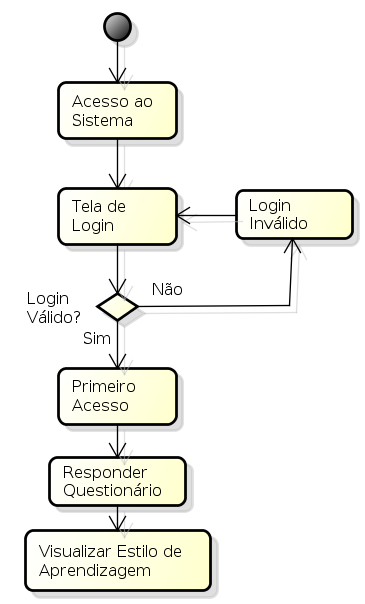
\includegraphics[scale=0.6]{images/fluxo-aluno.png}
	\caption{Fluxo de Execução para Experimentação do Perfil Aluno.}
	\label{fig:fluxo-aluno}
\end{figure}

A Figura~\ref{fig:frank-tela-aluno-inicial} apresenta o primeiro passo do fluxo do aluno, o acesso à tela inicial do Sistema, onde é mostrado uma mensagem de boas vindas. 

\begin{figure}
	\centering
	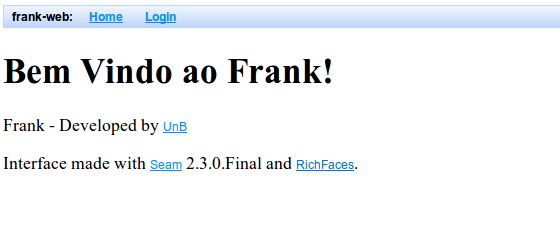
\includegraphics[scale=0.6]{images/frank-tela-aluno-inicial.png}
	\caption{Tela Inicial do Sistema.}
	\label{fig:frank-tela-aluno-inicial}
\end{figure}

O usuário prossegue para a tela de autenticação e o Sistema exige o login e a senha de acesso, apresentado na Figura~\ref{fig:frank-tela-aluno-login}. 

\begin{figure}
	\centering
	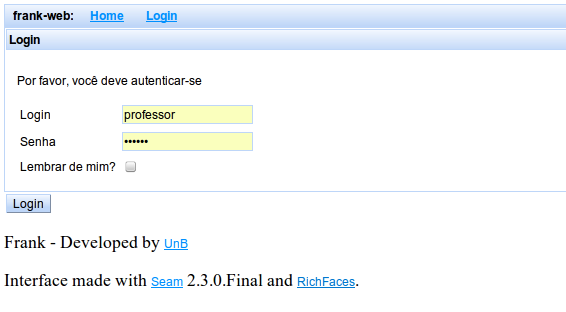
\includegraphics[scale=0.6]{images/frank-tela-aluno-login.png}
	\caption{Tela de Autenticação do Sistema.}
	\label{fig:frank-tela-aluno-login}
\end{figure}

Caso o usuário informe o login inválido, o Sistema apresenta a tela de erro, solicitando novamente os dados para autenticação. A Figura~\ref{fig:frank-tela-login-invalido} apresenta a tela de erro exibida para o usuário.

\begin{figure}
	\centering
	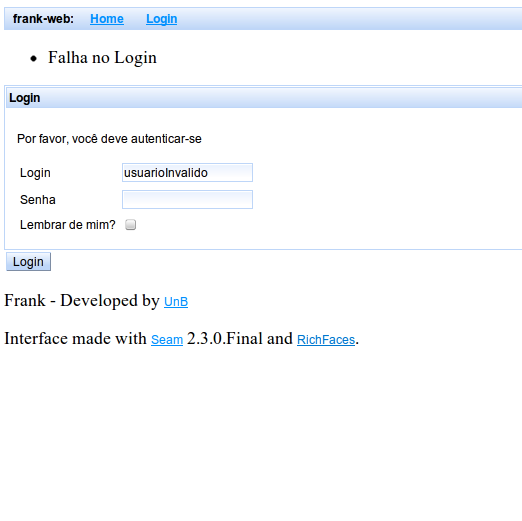
\includegraphics[scale=0.6]{images/frank-tela-login-invalido.png}
	\caption{Tela de Erro de Autenticação do Sistema.}
	\label{fig:frank-tela-login-invalido}
\end{figure}

Após a autenticação, a plataforma SMA cria o grupo de trabalho para o aluno. A Figura~\ref{fig:agente-rma-login-usuario} apresenta o agente grupo de trabalho (gt4) criado para o aluno 4 com os seguintes agentes de suporte: cognitivo (ac4), agente metacognitivo (am4), agente afetivo (aa4).
\begin{figure}
	\centering
	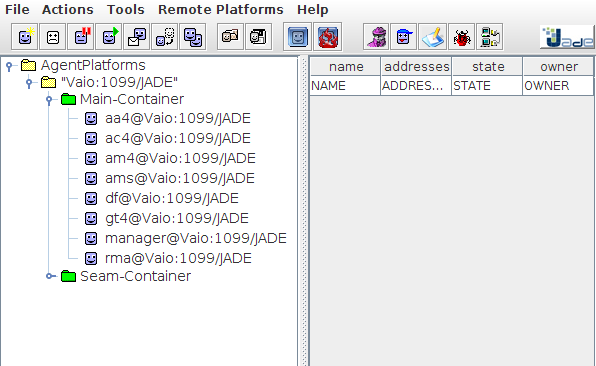
\includegraphics[scale=0.6]{images/agente-rma-login-usuario.png}
	\caption{Criação do grupo de trabalho para o Aluno 4.}
	\label{fig:agente-rma-login-usuario}
\end{figure}

Ao realizar o primeiro acesso ao Sistema, é detectado que o aluno não respondeu o questionário de estilos de aprendizagem. Assim, o Sistema apresenta a tela de convite para o seu preenchimento, conforme ilustra a Figura~\ref{fig:frank-tela-aluno-prim-acesso}.

\begin{figure}
	\centering
	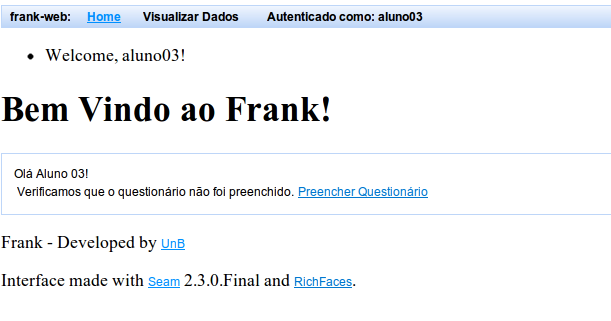
\includegraphics[scale=0.6]{images/frank-tela-aluno-prim-acesso.png}
	\caption{Tela de convite ao preenchimento do questionário de estilos de aprendizagem.}
	\label{fig:frank-tela-aluno-prim-acesso}
\end{figure}

O usuário então entra na tela de preenchimento do questionário, apresentada na Figura~\ref{fig:frank-tela-aluno-preencher-questionario}, responde o questionário de acordo com suas características e em seguida seleciona o botão ``Confirmar''. O Sistema envia os dados para o SMA onde o seu estilo de aprendizagem é mapeado.

\begin{figure}
	\centering
	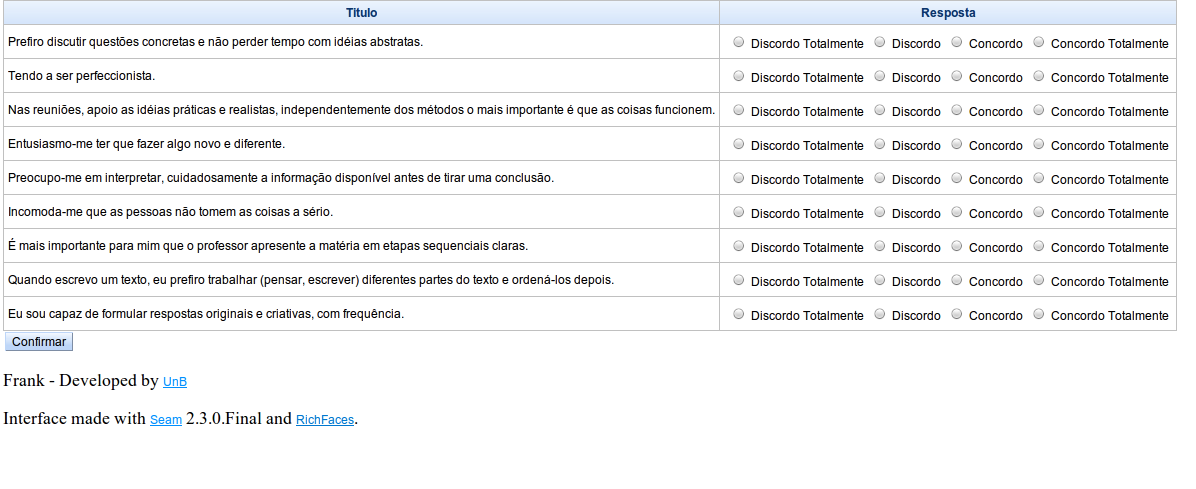
\includegraphics[scale=0.4]{images/frank-tela-aluno-preencher-questionario.png}
	\caption{Tela de prenchimento do questionário.}
	\label{fig:frank-tela-aluno-preencher-questionario}
\end{figure}

Por fim, o Sistema exibe o resultado final do processamento do SMA na tela de principal do aluno, exibido na Figura~\ref{fig:frank-tela-aluno-inferencia-estilo}. Dessa forma, o usuário verá sempre o seu estilo de aprendizagem atualizado ao acessar o Sistema.

\begin{figure}
	\centering
	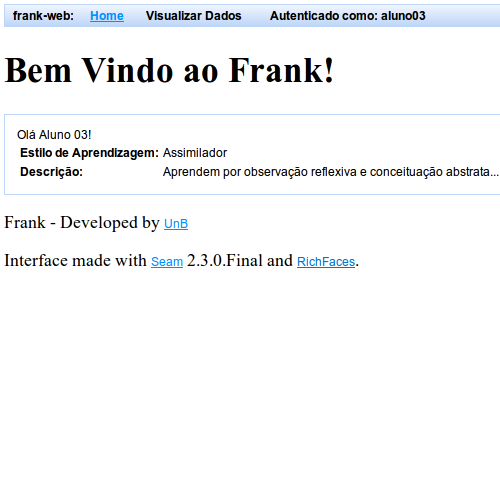
\includegraphics[scale=0.6]{images/frank-tela-aluno-inferencia-estilo.png}
	\caption{Tela de visualização do estilo de aprendizagem mapeado.}
	\label{fig:frank-tela-aluno-inferencia-estilo}
\end{figure}

\section{Apresentação da Interface com Docente}\label{section:interface-docente}

O fluxo apresentado na Figura~\ref{fig:fluxo-aluno} define a execução da experimentação do docente. Ele consiste do acesso à plataforma, sua autenticação, visualização das turmas e visualizar o estilo de aprendizagem dos alunos. Caso o seu login esteja incorreto, ele deve tentar novamente.

\begin{figure}
	\centering
	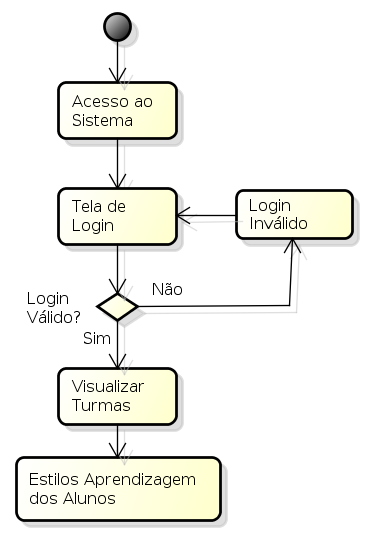
\includegraphics[scale=0.6]{images/fluxo-docente.png}
	\caption{Fluxo de Execução para Experimentação do Perfil Docente.}
	\label{fig:fluxo-aluno}
\end{figure}

É possível notar que o fluxo do docente é semelhante ao fluxo do aluno até a verificação de validade do login. O Sistema distingue os usuários neste momento e, no caso do Docente, renderiza uma tela diferente devido ao seu perfil. 

Após a autenticação do Docente o Sistema exibe a tela de visualização de turmas, apresentado na Figura~\ref{fig:frank-tela-professor-acesso}.

\begin{figure}
	\centering
	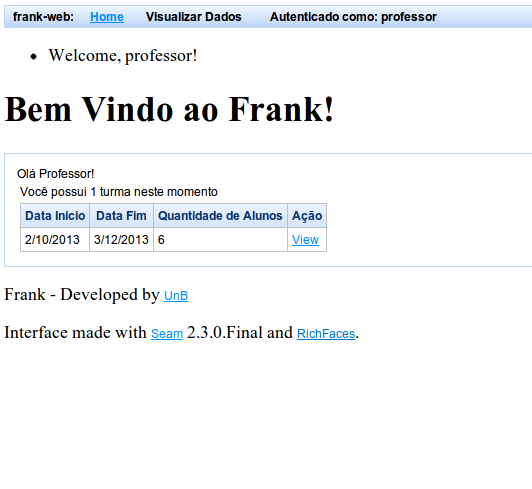
\includegraphics[scale=0.6]{images/frank-tela-professor-acesso.png}
	\caption{Tela inicial do usuário com o perfil de docente.}
	\label{fig:frank-tela-professor-acesso}
\end{figure}

O Docente seleciona a turma desejada e o Sistema aprensenta a tela de visualização de estilos de aprendizagem dos alunos pertencentes àquela turma. A Figura~\ref{fig:frank-tela-professor-visualizar-turma} apresenta um exemplo de visualização de estilos de aprendizagem da turma do Docente. É importante salientar que nem todos os alunos possuem um estilo de aprendizagem mapeado visto que, estes devem fazer acesso ao Sistema para o mapeamento do estilo ou, no futuro, podem possuir desvios no seu estilo de aprendizagem.

\begin{figure}
	\centering
	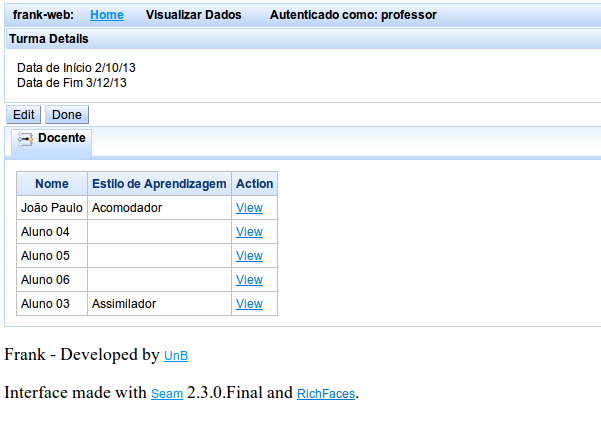
\includegraphics[scale=0.6]{images/frank-tela-professor-visualizar-turma.png}
	\caption{Tela de visualização do estilo de aprendizagem por turma.}
	\label{fig:frank-tela-professor-visualizar-turma}
\end{figure}

\section{Resultados}\label{section:resultados}
Após a execução das experimentações, foi possível observar vários aspectos do sistema. O primeiro deles é a assistência do aluno por meio do grupo de trabalho específico para ele, com os agentes cognitivo, metacognitivo e afetivo. Com esse grupo de trabalho será possível o mapeamento do seu modelo multidimensional por meio de dados de AVA.

Além disso, por meio de preenchimento de questionário e consequentemente a modelagem explícita, houve a determinação do seu estilo de aprendizagem. O agente cognitivo possui inteligência para interpretar as respostas do questionário e determinar o seu estilo de aprendizagem.

Por fim, através do cenário do docente, foi possível visualizar a notificação do estilo de aprendizagem dos seus alunos feito pela plataforma.

Neste capítulo foram apresentados os fluxos de utilização do sistema por meio de dois cenários: entidades Aluno e Docente. Em seguida, foram expostos os resultados obtidos por meio dos cenários e a forma como eles ajudam a atingir os objetivos. O próximo capítulo contém as conclusões e os trabalhos futuros.
